\subsubsection{MVC pattern}

    Our system will be strongly based on the MVC architectural pattern; this choice is due to the fact that this pattern will help us reducing the complexity of the structure of the system, by distributing all the functionalities between three interconnected parts (model, view and controller).
    \newline
    \newline
    The following schema explains this pattern:
    \begin{figure}[H]
            \centering
            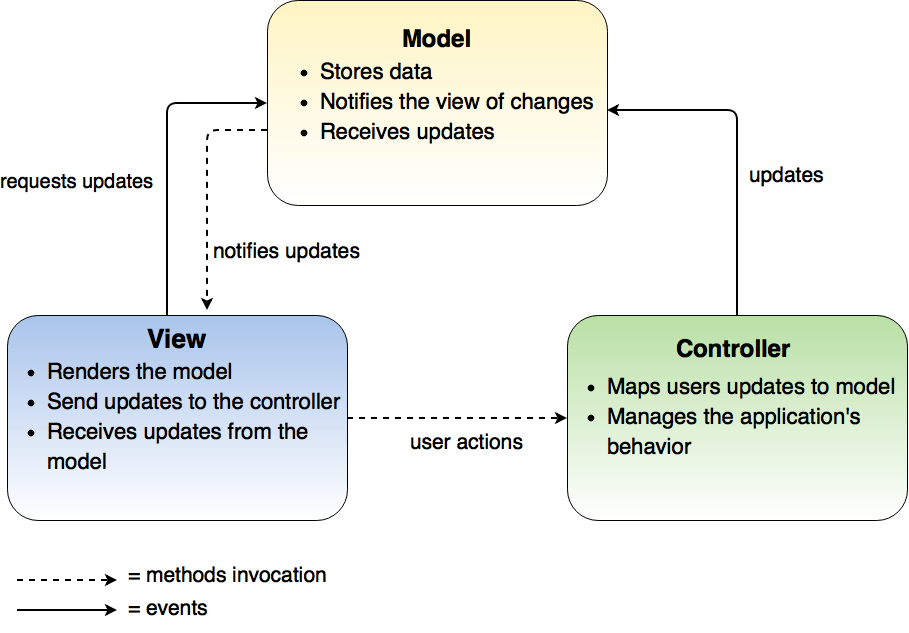
\includegraphics[width=15cm]{./Images/MVC.png}
            \caption{MVC pattern}
    \end{figure}

\subsubsection{Client-server model}

    In our project, we have referred to this model two times: for the communication between the clients and the web server and the one between the application server and the database.

\subsubsection{State pattern}

    This pattern will be used to manage the behaviour of the taxi drivers; indeed, taxi drivers will be provided with a status (that can be 'available', 'notAvailable' or 'offline' as discussed in the RASD\footnote{\label{note1}see the Class Diagram in the 'Specific Requirements' section}) and, according to their state, they will be able to perform only some specific actions.
    For example, if the status of a taxi driver is 'notAvailable', he will not be inserted in any queue and so he will be not allowed to accept any request.
    \newline
    Further, this pattern will be used also for request; each request has a status (that can be 'waiting', 'riding', 'completed' as discussed in the RASD\footnotemark[\ref{note1}]) and also in this case, according to the status of the request, only some specific kind of actions can be performed. For instance, if the status of a request is 'riding', it means that there must be a taxi driver associated to that request, while if a request is 'waiting' there are no taxi drivers associated to this request.

\subsubsection{Web services}